\documentclass[12pt,a4paper]{article}
\usepackage[utf8]{inputenc} %polskie znaki
\usepackage[T1]{fontenc}	%polskie znaki
\usepackage{amsmath}		%matematyczne znaczki :3
\usepackage{enumerate}		%Dodatkowe opcje do funkcji enumerate
\usepackage{geometry} 		%Ustawianie marginesow
\usepackage{graphicx}		%Grafika
\usepackage{wrapfig}		%Grafika obok textu
\usepackage{float}			%Allows H in fugire
\pagestyle{empty} 			%usuwa nr strony

\newgeometry{tmargin=2cm, bmargin=2cm, lmargin=2cm, rmargin=2cm} 

\begin{document}
	\begin{center}
		\LARGE Trygonometria - karta pracy
	\end{center}
	\vspace{1.5cm}
	\begin{tabular}{p{13cm} r}
		Imię i nazwisko: ............................................................................
		&[....../30pkt]\\ 
		\vspace{0.5cm}
	\end{tabular}
\newline
	\textbf{UWAGA:} Przez "wyznacz pozostałe funkcje trygonometryczne" rozumie się: sin, cos, tg i ctg.
	\begin{enumerate}[1.]
		
		\item  \begin{tabular}{p{13cm} r}
			Dany jest trójkąt prostokątny, w którym przeciwprostokątna wynosi 10, a jedna z przyprostokątnych 5. Wyznacz funkcje trygonometryczne wszystkich kątów ostrych tego trójkąta. &[4pkt]\\ 
		\end{tabular}
	
	\item \begin{tabular}{p{13cm} r}
		Oblicz brakujące boki: &[4pkt]\\ 
	\end{tabular}
	
	\begin{figure}[h]
		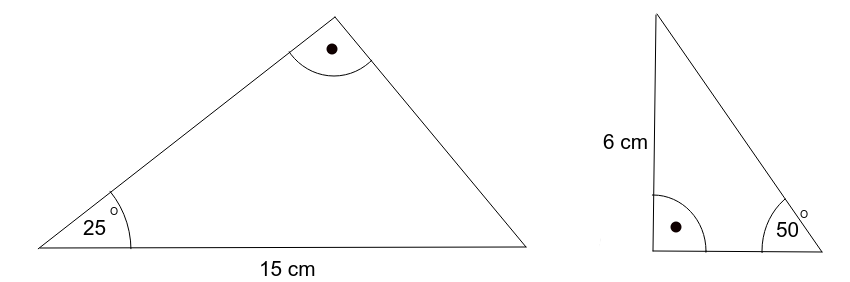
\includegraphics[scale=0.65]{tt1}
	\end{figure}
		
		\begin{tabular}{p{13cm} r}
			\item Dany jest $\cos \alpha = \frac{4}{5}$, dla pewnego kąta $\alpha \in (270^\circ, 360^\circ)$. Wyznacz jego pozostałe funkcje trygonometryczne. &[4pkt]\\ 
		\end{tabular}
	
	\begin{tabular}{p{13cm} r}
		\item Oblicz:
		\begin{enumerate}[a)]
			\item $\sin240^\circ=$
			\item $\cos(-420^\circ)=$
			\item $\sin120^\circ:\cos300^\circ=$
			\item $\text{tg } 135^\circ \cdot \text{ctg } 45^\circ=$
			\item $\sin15^\circ=$
		\end{enumerate}
		 &[8pkt]\\ 
	\end{tabular}
	
	\begin{tabular}{p{13cm} r}
		\item Dany jest trójkąt $ABC$, w którym bok $AB$ jest o 6 krótszy od boku $AC$ oraz $|BC|=5\sqrt{2}$. Wiedząc, że $\angle ABC = 135^\circ$: &[10pkt]\\ 
	\end{tabular}

	\begin{enumerate}[a)]
		\item Oblicz boki $AB$ i $AC$
		\item Oblicz pole tego trójkąta
		\item Wyznacz pozostałe kąty tego trójkąta
		\item Oblicz promień okręgu opisanego na tym trójkącie
	\end{enumerate}

	\end{enumerate}
	
\end{document}